% -----------------------------------------------------------------------------
\section{SBOL Data Model}\label{sec:model}
% -----------------------------------------------------------------------------

\Rtodo{All captions need full explanations.  JSB: done}
\Rtodo{Make sure all captions are sane and similar -JSB; JSB: done}

In this section, we describe the types of biological design data that can belong to an SBOL document and the relationships between these data types. The SBOL data model is specified using Unified Modeling Language (UML) 2.0 diagrams \href{http://www.omg.org/spec/UML/2.0/}{(OMG 2005)}. Subsections \ref{sec:umldiagrams}, \ref{sec:nameconventions}, \ref{sec:datatypes} review the basics of UML diagrams and explain the naming conventions and generic data types used in this specification. The remaining sections then describe the SBOL data model in detail. Complete SBOL examples and best practices when using the standard can be found in \ref{sec:examples} and \ref{sec:bestpractices}, respectively. 

\subsection{Understanding the UML Diagrams}
\label{sec:umldiagrams}

The types of biological design data modeled by SBOL are commonly referred to as {\em classes}, especially when discussing the details of software implementation. Each SBOL class can be instantiated by many SBOL objects. These objects may contain data that differ in content, but they MUST agree on the type and form of their data as dictated by their common class. Classes are represented in UML diagrams as rectangles labeled at the top with class names.

Classes may be connected to other classes by association properties, which are represented in UML diagrams as arrows. These arrows are labeled with data cardinalities in order to indicate how many values a given association property may possess (see below). The remaining (non-association) properties of a class are listed below its name. Each of the latter properties is labeled with its data type and cardinality.

In the case of an association property, the class from which the arrow originates is the owner of the association property. A diamond at the origin of the arrow indicates the type of association. Open-faced diamonds indicate shared aggregation, in which the owner of the association property exists independently of its value. In the SBOL data model, the value of an association property MUST be a URI or collection of URIs that refer to one or more SBOL objects belonging to the class at the tip of the arrow.

By contrast, filled diamonds indicate composite aggregation, also known as a part-whole relationship, in which the value of the association property MUST NOT exist independently of its owner. In addition, in the SBOL data model, it is REQUIRED that the value of each composite aggregation property is a unique SBOL object (that is, not the value for more than one such property).
%For example, it will later be shown how objects of the \sbol{SequenceAnnotation} class must associated with an object of the \sbol{ComponentDefinition} class (and only that object).

All SBOL properties are labeled with one of several restrictions on data cardinality. These are:

\begin{itemize}

\item $1$ - required, one: there must be exactly one value for this property.

\item $0 \ldots 1$ - optional: there may be a single value for this property or it may be absent.

\item $0 \ldots *$ - unbounded: there may be any number of values for this property, including none.

\item $1 \ldots *$ - required, unbounded: there may be any number of values for this property, as long as there is at least one.

\item $n \ldots *$ - at least: there must be at least $n$ values for this property.

\end{itemize}

Finally, classes can inherit the properties of other classes. Inheritance relationships are represented in UML diagrams as open-faced, triangular arrows that point from the inheriting class to the inherited class. Some classes in the SBOL data model cannot be instantiated as objects and exist only to group common properties for inheritance. These classes have italicized names and are known as abstract classes.

\subsection{Naming and Font Conventions}
\label{sec:nameconventions}

SBOL classes are named using upper "camel case," meaning that each word is capitalized and all words are run together without spaces e.g. \sbol{Identified}, \sbol{SequenceAnnotation}.  
Properties, on the other hand, are named using lower camel case, meaning that they begin lower case (e.g., \sbol{identity}) but if they consist of multiple words, all words after the first begin with an upper case letter (e.g., \sbol{persistentIdentity}).

Within the SBOL data model, each property is given a singular or plural name in accordance with its data cardinalities. The forms of these names follow the usual rules of grammar. For example, \sbol{SequenceAnnotation} is the singular form of \sbol{SequenceAnnotation}s. 

When SBOL objects are serialized to be exchanged (using \emph{Resource Description Framework} (RDF) as described in \ref{sec:serialization}), however, SBOL properties are always given singular names. This is because the SBOL data model does not contain classes that correspond directly to the RDF elements that group other elements into ordered or unordered sets. Consequently, if an SBOL property has multiple values, then it is serialized as multiple property entries, each with a singular name and a single value.
For example, if an SBOL property has five values, then its serialization contains five RDF triples, each with a singular predicate name and one of the five values as its object.

Lastly, font color is used in the body text of this specification to indicate whether a class or property is defined externally or within the SBOL data model. In particular, if a class or property name is written in a blue font, then it is defined by SBOL. If it is written in a bold font, then it is defined externally.

\subsection{Data Types}
\label{sec:datatypes}

\Ctodo{we use String, Integer, URI, Literal (these are from some W3C or XSD or whatever thing), and the classes below}
\Rtodo{Give a forward pointer to RECOMMENDED best-practices for compliant URIs.  JSB: done}

When SBOL use simple ``primitive'' data types such as strings or integers, these are defined as the following specific formal types:
\begin{itemize}
\item String: \url{http://www.w3.org/2001/XMLSchema#string}
\item Integer: \url{http://www.w3.org/2001/XMLSchema#integer}
\item URI: \url{something goes here}
  It is further RECOMMENDED that URI structure follows the recommended best-practices for compliant URIs specified in \ref{sec:compliant}..
\item Literal: \url{something goes here}
\end{itemize}

\subsection{Identified}
\label{sec:Identified}

\Ctodo{Put a small concrete example for each toplevel, in the style of the mapsTo diagram}

All SBOL-defined classes are directly or indirectly derived from the \sbol{Identified}  abstract class. This inheritance means that all SBOL objects are identified using \external{URI}s that uniquely refer to these objects within an SBOL document or at locations on the World Wide Web. 

As shown in \ref{uml:identified}, the \sbol{Identified} class includes the following properties: \sbol{identity}, \sbol{persistentIdentity},  \sbol{version}, \sbol{wasDerivedFrom}, \sbol{name}, \sbol{description}, and \sbol{annotations}. The latter property is described separately in \ref{sec:Annotations}.

When an SBOL object is referred to using a URI, that URI may either be the value of an \sbol{identity} property or to the value of a \sbol{persistentIdentity} property.
If the URI is equal to the value of an \sbol{identity} property, then it is guaranteed to be unique, and refers to precisely to one SBOL object with that value.
If the URI is equal to the value of a \sbol{persistentIdentity} property, then it may refer to multiple SBOL objects that are different ``versions'' of each other. These objects SHOULD be compared to one another to determine which single object the URI should be resolved to (usually the most recent version - see \ref{sec:version}).
Throughout this document, when a URI is used to refer to an SBOL object, it could fall into either of these cases.

\Rtodo{Remove ``identity'' for names of URIs everywhere.  JSB: done}


\begin{figure}[ht]
\begin{center}
\includegraphics[scale=0.6]{uml/identified}
\caption[]{Diagram of the \sbol{Identified} abstract class and its associated properties}
\label{uml:identified}
\end{center}
\end{figure}

\subsubsection*{The \sbolheading{identity} property}
\label{sec:identity}
The \sbol{identity} property is REQUIRED by all \sbol{Identified} objects and has a data type of \external{URI}. A given \sbol{Identified} object's \sbol{identity} \external{URI} MUST be globally unique among all other \sbol{identity} \external{URI}s. 

Although most SBOL properties are defined by SBOL and serialized with its namespace, the \sbol{identity} property is defined by the analogous RDF \external{about} property and is serialized with the RDF namespace as follows:

\external{http://www.w3.org/1999/02/22-rdf-syntax-ns\#about}.

This substitution is in keeping with the commitment of the SBOL community to the practical reuse of existing standards.

\subsubsection*{The \sbolheading{persistentIdentity} property}
\label{sec:persistentIdentity}
The \sbol{persistentIdentity} property is OPTIONAL and has a data type of \external{URI}. This \external{URI} serves to uniquely refer to a set of SBOL objects that are different versions of each other. 

An \sbol{Identified} object MUST be referred to using either its \sbol{identity} \external{URI} or its \sbol{persistentIdentity} \external{URI}.

\subsubsection*{The \sbolheading{displayId} property}
\label{sec:displayId}
The \sbol{displayId} property is an OPTIONAL identifier with a data type of \external{String}. This property is intended to be an intermediate between \sbol{name} and \sbol{identity} that is machine-readable, but more human-readable than the full \external{URI} of an \sbol{identity}. 

If the \sbol{displayId} property is used, then its \external{String} value SHOULD be locally unique (global uniqueness is not required) and MUST be compliant with the type \external{http://www.w3.org/TR/xmlschema-2/\#NCName}

\Ctodo{This is the wrong syntax.  It allows "-" and "." which we do not allow.  When resolving, make sure validation rules are in sync with the decision taken.}

\subsubsection*{The \sbolheading{version} property}
\label{sec:version}

The \sbol{version} property is OPTIONAL and has a data type of \external{String}. This property can be used to compare two SBOL objects with the same \sbol{persistentIdentity}.

If the \sbol{version} property is used, then it is RECOMMENDED that version numbering should follow the conventions of semantic versioning (\url{http://semver.org/}), particularly as implemented by Maven (\url{http://maven.apache.org/}).
This convention represents versions as sequences of numbers and qualifiers that are separated by the characters {\tt .} and {\tt -} and are compared in lexicographical order (for example, 1 < 1.3.1 < 2.0-beta).
For a full explanation, see the linked resources.

\subsubsection*{The \sbolheading{wasDerivedFrom} property}
\label{sec:wasDerivedFrom}

The \sbol{wasDerivedFrom} property is OPTIONAL and has a data type of \external{URI}. An SBOL object with this property refers to another SBOL object or non-SBOL resource from which this object was derived. 

If the \sbol{wasDerivedFrom} URI of an SBOL object $B$ refers to another SBOL object $A$ and either $B$ or $A$ has a \sbol{persistentIdentity}, then both $B$ and $A$ must have the same \sbol{persistentIdentity} \external{URI}. In addition, if both $B$ and $A$ have a \sbol{version}, then the \sbol{version} \external{String} of $A$ MUST come before that of $B$. Finally, an SBOL object MUST NOT refer to itself via its own  \sbol{wasDerivedFrom} property or form a circular chain of references via its \sbol{wasDerivedFrom} property and those of other SBOL objects (for example, the reference chain ``$B$ was derived from $A$ and $A$ was derived from $B$'' is circular).

\subsubsection*{The \sbolheading{name} property}
\label{sec:name}

\Ctodo{Need to require use of DublinCore names and show examples of them: non-stanard mappings per Matt: Title vs. Name, descripton is dcterms:description}

The \sbol{name} property is OPTIONAL and has a data type of \external{String}. This property is intended to be displayed to a human when visualizing an \sbol{Identified} object.

If an \sbol{Identified} object lacks a name, then software tools SHOULD instead display the object's \sbol{displayId} or \sbol{identity}.
It is RECOMMENDED that software tools give users the ability to switch perspectives between \sbol{name} properties that are human-readable and \sbol{displayId} properties that are less human-readable, but are more likely to be unique.

\subsubsection*{The \sbolheading{description} property}
\label{sec:description}

The \sbol{description} property is OPTIONAL and has a data type of \external{String}. This property is intended to contain a more thorough text description of an \sbol{Identified} object.

\subsubsection*{Serialization}

No complete serialization is defined for \sbol{Identified}, since this
class is only used indirectly through its child classes.  Any such
child class, however, has the following form for serializing
properties inherited from \sbol{Identified}, where CLASS\_NAME is
replaced by the name of the class:

\lstsetsbol
\begin{lstlisting}
<sbol:CLASS\_NAME rdf:about="...">
  [\emph{zero or one}]  <dcterms:title>...</dcterms:title> [\emph{element}]
  [\emph{zero or one}]  <dcterms:description>...</dcterms:description> [\emph{element}]
               ...
</sbol:CLASS\_NAME>
\end{lstlisting}

\Ctodo{Need somebody who knows DublinCore to fill in rest of template}

% \subsection{Documented}
% \label{sec:Documented}
% The \sbol{Documented} abstract class is inherited by the classes of SBOL objects that can contain human-readable properties, such as name and description. This class extends \sbol{Identified} with two additional data properties: \sbol{name}, and \sbol{description} (\ref{uml:documented}). 

% \begin{figure}[ht]
% \begin{center}
% \includegraphics[scale=0.6]{uml/documented}
% \caption[]{The \sbol{Documented} abstract class.}
% \label{uml:documented}
% \end{center}
% \end{figure}

% \subsubsection*{Serialization}

% No complete serialization is defined for \sbol{Documented}, since this
% class is only used indirectly through its child classes.  Any such
% child class, however, has the following form for serializing
% properties inherited from \sbol{Documented}, where CLASS\_NAME is
% replaced by the name of the class:

\subsection {TopLevel}
\label{sec:TopLevel}
\sbol{TopLevel} is an abstract class that is extended by any \sbol{Identified} class that can be found at the top level of an SBOL document or file. In other words, \sbol{TopLevel} objects are not nested inside any other object via a composite aggregation or black diamond arrow association property. Instead of nesting, composite \sbol{TopLevel} objects refer to subordinate \sbol{TopLevel} objects by their URIs using shared aggregation or white diamond arrow association properties. The \sbol{TopLevel} classes defined in this specification are \sbol{Sequence}, \sbol{ComponentDefinition}, \sbol{Model}, \sbol{ModuleDefinition},  \sbol{Collection}, and \sbol{GenericTopLevel} (\ref{uml:toplevel}).

\begin{figure}[ht]
\begin{center}
\includegraphics[width=\textwidth]{uml/toplevel}
\caption[]{Classes that inherit from the \sbol{TopLevel} abstract class.}
\label{uml:toplevel}
\end{center}
\end{figure}

\subsubsection*{Serialization}

No serialization is defined for \sbol{TopLevel}, since this class has
no properties of its own and is only used indirectly through its child
classes.

\subsection{Sequence}
\label{sec:Sequence}
The purpose of the \sbol{Sequence} class is to represent the primary structure of a \sbol{ComponentDefinition} object and the manner in which it is encoded. This representation is accomplished  by means of the \sbol{elements} property and \sbol{encoding} property (\ref{uml:sequence}).

\begin{figure}[ht]
\begin{center}
\includegraphics[scale=0.6]{uml/sequence}
\caption[]{Diagram of the \sbol{Sequence} class and its associated properties.}
\label{uml:sequence}
\end{center}
\end{figure}


\subsubsection*{The \sbolheading{elements} property}
\label{sec:elements}
The \sbol{elements} property is a REQUIRED \external{String} of characters that represents the constituents of a biological or chemical molecule. For example, these characters could represent the nucleotide bases of a molecule of DNA, the amino acid residues of a protein, or the atoms and chemical bonds of a small molecule.

\subsubsection*{The \sbolheading{encoding} property}
\label{sec:encoding}
The \sbol{encoding} property is REQUIRED and has a data type of \external{URI}. This property is used to indicate how the \sbol{elements} property of its \sbol{Sequence} object MUST be formed and interpreted.
For example, a \sbol{Sequence} object that represents a DNA sequence would have an \external{IUPAC DNA} encoding that requires the \sbol{elements} property to contain characters that represent nucleotide bases, such as {\tt a}, {\tt t}, {\tt c}, and {\tt g}. A \sbol{Sequence} object that represents the chemical structure of glucose, however, might have a \external{simplified molecular-input line-entry system (SMILES)} encoding that requires the \sbol{elements} property to contain characters that represent atoms and chemical bonds, such as {\tt C}, {\tt N}, {\tt O}, and {\tt =}.

\ref{tbl:sequence_encodings} provides a list of RECOMMENDED \external{URI}s for the \sbol{encoding} property. When the \sbol{encoding} of a \sbol{Sequence} is well described by one of the \external{URI}s in \ref{tbl:sequence_encodings}, it SHOULD use that \external{URI} for this property.

%A Summary of letters for nucleic acids and aminoacids
\begin{table}[ht]
  \begin{edtable}{tabular}{lll}
    \toprule
     \textbf{Encoding} & \textbf{URI} & \textbf{ComponentDefinition Type} \\
    \midrule
     IUPAC DNA, RNA & \url{http://www.chem.qmul.ac.uk/iubmb/misc/naseq.html} & DnaRegion,RnaRegion \\
    IUPAC Protein & \url{http://www.chem.qmul.ac.uk/iupac/AminoAcid/} & Protein\\
   SMILES & \url{http://www.opensmiles.org/opensmiles.html} & SmallMolecule \\
    \bottomrule
  \end{edtable}
  \caption{The RECOMMENDED \external{URI}s for encoding the \sbol{Sequence} objects for common types of \sbol{ComponentDefinition} (see \ref{tbl:componentdefinition_types}).}
  \label{tbl:sequence_encodings}
\end{table}

\subsubsection*{Serialization}
The serialization of a \sbol{Sequence} object has the following form:
\lstsetsbol
\begin{lstlisting}
<sbol:Sequence rdf:about="...">
      ...
  [\emph{one}] <sbol:elements>...</sbol:elements> [\emph{element}]
  [\emph{one}] <sbol:encoding rdf:resource="..."/> [\emph{element}]
</sbol:Sequence>
\end{lstlisting}

The example below shows the serialization of the \sbol{Sequence} object for the \sbol{ComponentDefinition} of a promoter. The nucleotide bases of the \sbol{Sequence} are serialized as the \external{String} value for its \sbol{elements} property, while its \external{IUPAC DNA} encoding is serialized as the \external{URI} value for its  \sbol{encoding} property. 

\lstsetsbol
\begin{lstlisting}
<sbol:Sequence rdf:about="http://www.partsregistry.org/Part:BBa_J23119:Design">
  <sbol:elements>ttgacagctagctcagtcctaggtataatgctagc</sbol:elements>
  <sbol:encoding rdf:resource="http://www.chem.qmul.ac.uk/iubmb/misc/naseq.html"/>
</sbol:Sequence>
\end{lstlisting}


\subsection{ComponentDefinition}
\label{sec:ComponentDefinition}

The \sbol{ComponentDefinition} class represents the structural entities of a biological design. The primary usage of this class is to represent structural entities with designed sequences, such as DNA, RNA, and proteins, but it can also be used to represent any other entity that is part of a design, such as small molecules, molecular complexes, and light. 

As shown in \ref{uml:component_definition}, the \sbol{ComponentDefinition} class describes a structural design entity using the following properties: \sbol{types}, \sbol{roles}, and \sbol{sequences}. In addition, this class has properties for describing and organizing the substructure of said design entity, including \sbol{components}, \sbol{sequenceConstraints}, and  \sbol{sequenceAnnotations}.

\Rtodo{Make sure that text is consistent with sequences property have cardinality of 0..*; JSB: done}

\begin{figure}[ht]
\begin{center}
\includegraphics[width=0.95\textwidth]{uml/component_definition}
\caption[]{Diagram of the \sbol{ComponentDefinition} class and its associated properties.}
\label{uml:component_definition}
\end{center}
\end{figure}

\subsubsection*{The \sbolheading{types} property}
\label{sec:types}

The \sbol{types} property is a REQUIRED set of \external{URI}s that specifies the category of biochemical or physical entity (for example DNA, protein, or small molecule) that a \sbol{ComponentDefinition} object abstracts for the purpose of engineering design. 

The \sbol{types} property of every \sbol{ComponentDefinition} MUST contain at least one \external{URI} that SHOULD identify a term from an appropriate ontology, such as the BioPAX ontology or the ontology of Chemical Entities of Biological Interest (ChEBI). \ref{tbl:componentdefinition_types} provides a list of RECOMMENDED ontology terms for the \sbol{types} property and their \external{URI}s. In order to maximize the compatibility of designs, any \sbol{ComponentDefinition} that can be well-described by one of the terms in \ref{tbl:componentdefinition_types} SHOULD use that term as one of its \sbol{types}. Finally, if the \sbol{types} property contains multiple \external{URIs}, then they SHOULD identify synonymous terms. 

\begin{table}[ht]
  \begin{edtable}{tabular}{ll}
    \toprule
    \textbf{ComponentDefinition Type} & \textbf{URI for BioPAX Term} \\
    \midrule
    DNA  & \url{http://www.biopax.org/release/biopax-level3.owl#DnaRegion}\\
    RNA  & \url{http://www.biopax.org/release/biopax-level3.owl#RnaRegion}\\
    Protein  & \url{http://www.biopax.org/release/biopax-level3.owl#Protein}\\
    Small Molecule  & \url{http://www.biopax.org/release/biopax-level3.owl#SmallMolecule}\\  
    \bottomrule
  \end{edtable}
  \caption{RECOMMENDED BioPAX terms to specify the \sbol{types} property of a \sbol{ComponentDefinition}.}
  \label{tbl:componentdefinition_types}
\end{table}

\subsubsection*{The \sbolheading{roles} property}
\label{sec:roles}

The \sbol{roles} property is a OPTIONAL set of \external{URI}s that clarifies the potential function of a \sbol{ComponentDefinition} in a biological context.

The \sbol{roles} property of a \sbol{ComponentDefinition} MAY contain a collection of \external{URI}s that SHOULD identify terms from ontologies that are consistent with the \sbol{types} property of the \sbol{ComponentDefinition}. For example, the \sbol{roles} property of a DNA or RNA \sbol{ComponentDefinition} component SHOULD contain \external{URI}s identifying terms from the Sequence Ontology (SO). \ref{tbl:componentdefinition_roles} contains a list of RECOMMENDED ontology terms for the \sbol{roles} property and their \external{URI}s. These terms are organized by the type of \sbol{ComponentDefinition} to which they SHOULD apply. As with the \sbol{types} property, any \sbol{ComponentDefinition} that can be well-described by one of the terms in \ref{tbl:componentdefinition_roles} SHOULD use that term as one of its \sbol{roles}.

\begin{table}[ht]
  \begin{edtable}{tabular}{lll}
    \toprule
    \textbf{ComponentDefinition Role} & \textbf{URI for Ontology Term} & \textbf{ComponentDefinition Type} \\
    \midrule
   Promoter & \url{http://identifiers.org/so/SO:0000167} & DNA \\
   Ribosome Entry Site & \url{http://identifiers.org/so/SO:0000139} & DNA \\
      CDS & \url{http://identifiers.org/so/SO:0000316} & DNA \\
      Terminator & \url{http://identifiers.org/so/SO:0000141} & DNA \\ 
      Gene & \url{http://identifiers.org/so/SO:0000704} & DNA \\
      mRNA & \url{http://identifiers.org/so/SO:0000234} & RNA \\ 
      Transcription Factor & \url{http://identifiers.org/go/GO:0003700} & Protein \\
      Effector & \url{http://identifiers.org/chebi/CHEBI:35224} & Small Molecule \\
    \bottomrule
  \end{edtable}
  \caption{RECOMMENDED ontology terms to specify the \sbol{roles} property of a \sbol{ComponentDefinition}.}
  \label{tbl:componentdefinition_roles}
\end{table}

\subsubsection*{The \sbolheading{components} property}
\label{sec:components}

The \sbol{components} property is OPTIONAL and MAY specify a collection of \sbol{Component} objects contained by its \sbol{ComponentDefinition}.

While the \sbol{ComponentDefinition} class is analogous to a blueprint or specification sheet for a biological part, the \sbol{Component} class represents the specific occurrence of parts within a design. Hence, this class allows a biological design to include multiple copies of a particular part. For example, the \sbol{ComponentDefinition} of a gene MAY contain two \sbol{Component} objects that refer to the same \external{URI} for the \sbol{ComponentDefinition} of a CDS.

\subsubsection*{The \sbolheading{sequences} property}
\label{sec:sequences}
The \sbol{sequences} property is OPTIONAL and MAY include a collection of \external{URI}s for \sbol{Sequence} objects. These objects define the primary structure of the \sbol{ComponentDefinition} with this property and SHOULD be consistent with each other.

\Rtodo{Please check that this constraint is appropriate -JSB}
Many \sbol{Component} objects will have precisely one \sbol{Sequence} object in this collection.  In certain use cases, however, it may be appropriate to have multiple \sbol{Sequence} objects (e.g., two different representations of the same object), and accordingly multiple objects are permitted.  If there is more than one \sbol{Sequence}, however, it must be the case that their length and topology are precisely the same, such that it is unambiguous what is referred to be \sbol{SequenceConstraint} and \sbol{SequenceAnnotation} objects.

\subsubsection*{The \sbolheading{sequenceConstraints} property}
\label{sec:sequenceConstraints}

The \sbol{sequenceConstraints} property is OPTIONAL and MAY contain a collection of \sbol{SequenceConstraint} objects. These objects describe any restrictions on the relative, sequence-based positions of \sbol{Component} objects that belong to the \sbol{ComponentDefinition}.

\subsubsection*{The \sbolheading{sequenceAnnotations} property}
\label{sec:sequenceAnnotations}

The \sbol{sequenceAnnotations} property is OPTIONAL and MAY contain a collection of \sbol{SequenceAnnotation} objects. These objects describe  \sbol{Location}s on the \sbol{Sequence} objects of the  \sbol{ComponentDefinition}. In addition, each \sbol{SequenceAnnotation} can  position a \sbol{Component} of the \sbol{ComponentDefinition} at its specified \sbol{Location}.

\subsubsection*{Serialization}
% The parent classes of the \sbol{ComponentDefinition} class are \sbol{TopLevel} and, transitively, \sbol{Identified}. As a result, inherited properties are serialized as explained for these parent classes.
The \sbol{sequences}, \sbol{components},  \sbol{sequenceConstraints}, and \sbol{sequenceAnnotations} properties of a \sbol{ComponentDefinition} include \external{URI}s that identify objects belonging to the appropriate SBOL classes, while the \sbol{types} and \sbol{roles} properties include URIs that identify ontology terms. As shown in the example below, each of these URIs is serialized as an \external{rdf:resource} as part of an implicit collection of SBOL properties with singular rather then plural names.

\Rtodo{The name (title) and description properties should be moved from this example to one for Identified. Identified is an abstract class that shouldn't be serialized, but perhaps we could use a non-abstract class (probably ComponentDefinition) to provide an example of displayId, version, name, description, etc. - Nic;  JSB: moved forward}

\lstsetsbol
\begin{lstlisting}
<sbol:ComponentDefinition rdf:about="...">
               ...
  [\emph{zero or more}]  <sbol:sequence rdf:resource="..."/> [\emph{element}]
  [\emph{one or more}]  <sbol:type rdf:resource="..."/> [\emph{elements}]
  [\emph{zero or more}]  <sbol:role rdf:resource="..."/> [\emph{elements}]    
  [\emph{zero or more}] <sbol:component>
                 <sbol:Component rdf:about="...">...</sbol:Component>
               </sbol:component> [\emph{elements}]
  [\emph{zero or more}] <sbol:sequenceAnnotation>
                 <sbol:SequenceAnnotation rdf:about="...">...</sbol:SequenceAnnotation>
               </sbol:sequenceAnnotation> [\emph{elements}]        
  [\emph{zero or more}] <sbol:sequenceConstraint>
                 <sbol:SequenceConstraint rdf:about="...">...</sbol:SequenceConstraint>
               </sbol:sequenceConstraint> [\emph{elements}]        
</sbol:ComponentDefinition>
\end{lstlisting}
\Rtodo{We need to have an explanation of how to interpret these, and also have a pointer to it from each example.  JSB: I think the serialization section is enough, actually, and that these are relatively intuitive}

The example below shows the serialization of a simple \sbol{ComponentDefinition} for a promoter. The BioPAX term \external{DnaRegion} and the ChEBI term \external{CHEBI:4705} (\external{double-stranded DNA}) are used to indicate that the type of biological entity represented by this \sbol{ComponentDefinition} is DNA. Its role is specified using the SO terms \external{SO:0000167} (\external{promoter}) and the more specific \external{SO:0000613} (\external{bacterial\_RNApol\_promoter}).

\lstsetsbol
\begin{lstlisting}
<sbol:ComponentDefinition rdf:about="http://www.partsregistry.org/Part:BBa_J23119">
  <dcterms:title>J23119 promoter</dcterms:title>
  <dcterms:description>Constitutive promoter</dcterms:description>
  <sbol:type rdf:resource="http://identifiers.org/chebi/CHEBI:4705"/>
  <sbol:type rdf:resource="http://www.biopax.org/release/biopax-level3.owl#DnaRegion"/>
  <sbol:role rdf:resource="http://identifiers.org/so/SO:0000167"/>
  <sbol:role rdf:resource="http://identifiers.org/so/SO:0000613"/>
  <sbol:sequence rdf:resource="http://www.partsregistry.org/Part:BBa_J23119:Design"/>
</sbol:ComponentDefinition>
\end{lstlisting}


\subsubsection{ComponentInstance}
\label{sec:ComponentInstance}

\begin{figure}[ht]
\begin{center}
\includegraphics[scale=0.6]{uml/component_instance}
\caption[]{Diagram of the \sbol{ComponentInstance} class and its associated properties.}
\label{uml:component}
\end{center}
\end{figure}
\Ctodo{Nic, please change definition to componentDefinition in the diagram to match the text.}

When a \sbol{ComponentDefinition} is used as an element of a larger design, each separate usage is represented by a \sbol{ComponentInstance} object.  
The \sbol{ComponentInstance} class is abstract, so every usage must belong to one of its two subclasses:
\begin{itemize}
\item The \sbol{Component} class is used to specify the structural usage of a \sbol{ComponentDefinition} inside another \sbol{ComponentDefinition} via the \sbol{components} property.
\item The \sbol{FunctionalComponent} class is used to specify the functional usage of a \sbol{ComponentDefinition} inside a \sbol{ModuleDefinition} via the \sbol{functionalComponents} property. This class is described in \ref{sec:FunctionalComponent}.
\end{itemize}

\paragraph{The \sbolheading{componentDefinition} property}
\label{sec:componentDefinition}

Every \sbol{ComponentInstance} MUST be associated with precisely one
\sbol{ComponentDefinition}, which is the design that it is an instance of.

\paragraph{The \sbolheading{mapsTo} property}
\label{sec:mapsTo}

\Rtodo{Need to make sure all MapsTo statements are correct; JSB: done}
The \sbol{mapsTo} property links \sbol{Component} objects (both Components and FunctionalComponents) together within a larger design, indicating that they refer to the same entity.

The third data field, \sbol{mapsTo}, is a set of \sbol{MapsTo} objects.  These are used as described below in the section on \sbol{MapsTo} below, to identify definition relationships between other \sbol{ComponentInstance} objects.

\paragraph{The \sbolheading{access} property}
\label{sec:access}

The \sbol{access} determines whether a \sbol{ComponentInstance} 
can be identified with a part in a larger design via \sbol{MapsTo}.
The \sbol{access} property must be set to one of the following URIs:

\begin{itemize}
\item \url{http://sbols.org/v2#public}
  If the access is public, the \sbol{ComponentInstance} MAY be linked to by \sbol{MapsTo} objects.

\item \url{http://sbols.org/v2#private}
  If the access is private, the \sbol{ComponentInstance} MUST NOT be linked by any \sbol{MapsTo} object.
\end{itemize}

\paragraph{Serialization}

No serialization is defined for \sbol{ComponentInstance}, since this class is 
only used indirectly through its child classes.


\subsubsection{Component}
\label{sec:Component}
Composition of the structural layer of SBOL designs is accomplished using \sbol{Component} objects. Each \sbol{Component} instance is part of a \sbol{ComponentDefinition} object, associated with it by the \sbol{components} property to represent  physical composition.  

All \sbol{Component} objects directly referenced within a \sbol{ComponentDefinition}'s \sbol{SequenceAnnotation} or \sbol{SequenceConstraint} parts MUST be associated with that \sbol{ComponentDefinition} by means of its \sbol{components} property.

\paragraph{Serialization}

The serialization of a \sbol{ComponentInstance} object has the following form:

\lstsetsbol
\begin{lstlisting}
<sbol:Component rdf:about="...">
               ...
  [\emph{one}]           <sbol:access rdf:resource="..."/> [\emph{element}]
  [\emph{one}]           <sbol:definition rdf:resource="..."/> [\emph{elements}]    
  [\emph{zero or more}]  <sbol:mapsTo rdf:resource="..."/> [\emph{elements}]
</sbol:Component>
\end{lstlisting}

The example below shows the serialization of a \sbol{Component}
representing an instance of promoter:

\lstsetsbol
\begin{lstlisting}
<sbol:Component rdf:about="http://www.partsregistry.org/Part:BBa_F2620/pLuxR">
  <sbol:access rdf:resource="http://sbols.org/v2#public"/>
  <sbol:definition rdf:resource="http://www.partsregistry.org/Part:BBa_R0062"/>
</sbol:Component>
\end{lstlisting}


\subsubsection{SequenceAnnotation}
\label{sec:SequenceAnnotation}
The \sbol{SequenceAnnotation} class describes a precisely known location of interest on the \sbol{Sequence} objects linked by its parent \sbol{ComponentDefinition} object.  It can also optionally associate this location with a \sbol{Component} object. \sbol{SequenceAnnotation} objects specify their location using a \sbol{Location} object, as described below.

\Rtodo{We will change location to locations (1..*) and eliminate MultiRange class.  JSB, Nic: done}

\begin{figure}[ht]
\begin{center}
\includegraphics[scale=0.6]{uml/sequence_annotation}
\caption[]{Diagram of the \sbol{SequenceAnnotation} class and its associated properties.}
\label{uml:sequence_annotation}
\end{center}
\end{figure}

\paragraph{The \sbolheading{locations} property}\label{sec:locations}
\label{sec:locations}
Every \sbol{SequenceAnnotation} MUST has at least one \sbol{Location} object in its collection of \sbol{locations}. The value of this property is a nested \sbol{Location} object.

\paragraph{The \sbolheading{component} property}\label{sec:component}
\sbol{SequenceAnnotation} objects MAY use this property to link location information to a \sbol{Component} object, by specifying its URI.

\Rtodo{Separate serialization better - give paragraph/subsubsec headers.  JSB: done.}

\paragraph{Serialization}

The serialization of SequenceAnnotation objects MUST be carried out according to the template below. In this template, A\_LOCATION\_SUBCLASS represents one of the Location subclasses.
\lstsetsbol
\begin{lstlisting}
<sbol:SequenceAnnotation rdf:about="...">
               ...   
  [\emph{zero or one}] <sbol:component rdf:resource="..."/> [\emph{element}] 
  [\emph{one}]         <sbol:location>
                 <sbol:A_LOCATION_SUBCLASS rdf:about="...">...</sbol:A_LOCATION_SUBCLASS>
               </sbol:location> [\emph{element}] 
</sbol:SequenceAnnotation>
\end{lstlisting}

The example below shows the serialization of a \sbol{SequenceAnnotation} object. It specifies the location of a particular \sbol{Component} named BBa\_F2620.
\lstsetsbol
\begin{lstlisting}
    <sbol:sequenceAnnotation>
      <sbol:SequenceAnnotation rdf:about="http://www.partsregistry.org/Part:BBa_F2620/anno2">
        <sbol:location>
          <sbol:Range rdf:about="http://www.partsregistry.org/Part:BBa_F2620/anno2/range">
            <sbol:start>56</sbol:start>
            <sbol:end>68</sbol:end>
            <sbol:orientation rdf:resource="http://sbols.org/v2#inline"/>
          </sbol:Range>
        </sbol:location>
        <sbol:component rdf:resource="http://www.partsregistry.org/Part:BBa_F2620/rbs"/>
      </sbol:SequenceAnnotation>
    </sbol:sequenceAnnotation>
\end{lstlisting}

\Rtodo{Need to give an example with this one.  JSB: done.}

\Rtodo{Make sure it's clear these templates specify content, not order.  JSB: put a note explaining ordering is flexible in the serialization section.}



\subsubsection{Location}
\label{sec:Location}
The Location class is extended by the \sbol{Range}, \sbol{Cut}, and \sbol{GenericLocation} classes.  All of these thus share its \sbol{orientation} property, for example to to specify directionality on a potentially double-stranded \sbol{Component} object.

\begin{figure}[ht]
\begin{center}
\includegraphics[scale=0.6]{uml/location}
\caption[]{Diagram of the \sbol{Location} class and its associated properties.}
\label{uml:location}
\end{center}
\end{figure}

\subparagraph{The \sbolheading{orientation} property}
\label{sec:orientation}
This OPTIONAL property has a URI value. For \sbol{ComponentDefinition} objects representing DNA molecules, it is RECOMMENDED to use one of the values in \ref{tbl:orientation_types}. 

\begin{table}[ht]
  \begin{edtable}{tabular}{l}
    \toprule
    \textbf{Orientation Types}  \\
    \midrule
    http://sbols.org/v2\#inline\\
    http://sbols.org/v2\#reverseComplement\\
    \bottomrule
  \end{edtable}
  \caption{URI constants for \sbol{orientation} values}
  \label{tbl:orientation_types}
\end{table}


\paragraph{Range}
\label{sec:Range}
A \sbol{Range} object specifies inclusive start and end positions. These properties are required in \sbol{Range} objects and they can have \external{integer} values greater than zero.

\subparagraph{The \sbolheading{start} property}\label{sec:start}
Specifies the start of a \sbol{Range}. This property is REQUIRED and can have \external{integer} values greater than zero.

\subparagraph{The \sbolheading{end} property}\label{sec:end}
Specifies the end of a \sbol{Range}. This property is REQUIRED and can have \external{integer} values greater than zero.

\Rtodo{If we remove MultiRange than Orientation can be moved to the Location class.  Done: Nic and JSB}

\subparagraph{Serialization}

The serialization of Range objects has the following form:
\lstsetsbol
\begin{lstlisting}
<sbol:Range rdf:about="...">
               ...   
  [\emph{one}]         <sbol:start>...</sbol:start> [\emph{element}] 
  [\emph{one}]         <sbol:end>...</sbol:end> [\emph{element}] 
  [\emph{zero or one}] <sbol:orientation rdf:resource="..."/> [\emph{element}] 
</sbol:Range>
\end{lstlisting}

The example below shows the serialization of a \sbol{Range} object. It specifies the region between 56 and 68, and the orientation is given as \external{inline}.
\lstsetsbol
\begin{lstlisting}
<sbol:Range rdf:about="http://www.partsregistry.org/Part:BBa_F2620/anno2/range">
  <sbol:start>56</sbol:start>
  <sbol:end>68</sbol:end>
  <sbol:orientation rdf:resource="http://sbols.org/v2#inline"/>
</sbol:Range>
\end{lstlisting}

\paragraph{Cut}
\label{sec:Cut}
The \sbol{Cut} class has been introduced to enable the specification of a location between two indices. 
Each \sbol{Cut} object has the property \sbol{at}.

\subparagraph{The \sbolheading{at} property}
\label{sec:at}
The REQUIRED \sbol{at} property is an index greater than or equal to zero that specifies the index just before the location represented by the Cut object. 
A Cut object with \sbol{at} equal to zero represents the location just before index one (even though there is no zero index on Structure objects in SBOL). 

\subparagraph{Serialization}

The serialization of \sbol{Cut} objects has the following form:
\lstsetsbol
\begin{lstlisting}
<sbol:Cut rdf:about="...">
               ...   
  [\emph{one}]         <sbol:at>...</sbol:at> [\emph{element}] 
  [\emph{zero or one}] <sbol:orientation rdf:resource="..."/> [\emph{element}] 
</sbol:Cut>
\end{lstlisting}

The example below shows the serialization of a \sbol{Cut} object. It specifies the location after 27, and the orientation is given as \external{inline}.
\lstsetsbol
\begin{lstlisting}
<sbol:Cut rdf:about="http://www.partsregistry.org/Part:BBa_F2620/anno3/cut">
  <sbol:at>27</sbol:at>
  <sbol:orientation rdf:resource="http://sbols.org/v2#inline"/>
</sbol:Cut>
\end{lstlisting}


\paragraph{GenericLocation}
\label{sec:GenericLocation}

While the \sbol{Range} and \sbol{Cut} classes are best suited to
describing locations on sequential structures, the
\sbol{GenericLocation} is included as a hook for extensions, e.g., for
describing locations in non-sequential structures.

\Rtodo{Need serialization examples, Cut, and GenericLocation: JSB - done for Cut and GenericLocation}

\subparagraph{Serialization}

The serialization of \sbol{GenericLocation} objects has the following form:
\lstsetsbol
\begin{lstlisting}
<sbol:GenericLocation rdf:about="...">
               ...   
  [\emph{one}]         <sbol:at>...</sbol:at> [\emph{element}] 
  [\emph{zero or one}] <sbol:orientation rdf:resource="..."/> [\emph{element}] 
</sbol:GenericLocation>
\end{lstlisting}

The example below shows the serialization of a \sbol{GenericLocation} object with a reverse orientation:
\lstsetsbol
\begin{lstlisting}
<sbol:GenericLocation rdf:about="http://www.partsregistry.org/Part:BBa_F2620/anno5/location">
  <sbol:orientation rdf:resource="http://sbols.org/v2#reverseComplement"/>
</sbol:GenericLocation>
\end{lstlisting}

\subsubsection{SequenceConstraint}
\label{sec:SequenceConstraint}
A \sbol{ComponentDefinition} object can link to \sbol{SequenceConstraint} objects to assert various kinds of structural restrictions between two \sbol{Component} objects that are its subcomponents. 
The purpose of \sbol{SequenceConstraint} is to allow partial designs to be specified when the precise identity, location, or ordering of \sbol{Component} objects is not yet fully determined.

A \sbol{SequenceConstraint} object requires \sbol{restriction}, \sbol{subject} and \sbol{object} properties to specify such constraints.

\begin{figure}[ht]
\begin{center}
\includegraphics[scale=0.6]{uml/sequence_constraint}
\caption[]{Diagram of the \sbol{SequenceConstraint} class and its associated properties.}
\label{uml:sequence_constraint}
\end{center}
\end{figure}

\paragraph{The \sbolheading{subject} property}\label{sec:subject}
\label{sec:subject}
This REQUIRED property specifies the URI of the first \sbol{Component} object in the relation.

\paragraph{The \sbolheading{object} property}\label{sec:object}
\label{sec:object}
This REQUIRED property specifies the URI of the second \sbol{Component} object in the relation.

\paragraph{The \sbolheading{restriction} property}\label{sec:restriction}
\label{sec:restriction}

This REQUIRED property specifies a URI that identifies the type of relationship between the \sbol{subject} and \sbol{object} \sbol{Component} objects. 
The RECOMMENDED values for this property are given in \ref{tbl:restriction_types}.

Note: With regards to SBOL Version 1.1., this is a generalization of former \sbol{SequenceAnnotation} property \external{precedes}.

\begin{table}[ht]
  \begin{edtable}{tabular}{ll}
    \toprule
    \textbf{Restriction Types} & Subject/Object Relation \\
    \midrule
    http://sbols.org/v2\#precedes & Subject location is strictly less than object location \\
    http://sbols.org/v2\#sameOrientationAs & Subject and object have equal orientation URIs\\
    http://sbols.org/v2\#oppositeOrientationAs & Object orientation is ``opposite'' of subject\\    
    \bottomrule
  \end{edtable}
  \caption{URI constants for \sbol{restriction} values}
  \label{tbl:restriction_types}
\end{table}

\NVtodo{We need things like nextTo and overlapping, and think we might be able to get it from region-connection-calculus ontology}

\paragraph{Serialization}

The serialization of \sbol{SequenceConstraint} objects has the following form:
\lstsetsbol
\begin{lstlisting}
<sbol:SequenceConstraint rdf:about="...">
      ...
  [\emph{one}] <sbol:restriction rdf:resource="..."/> [\emph{element}]
  [\emph{one}] <sbol:subject rdf:resource="..."/> [\emph{element}]
  [\emph{one}] <sbol:object rdf:resource="..."/> [\emph{element}]
</sbol:SequenceConstraint>
\end{lstlisting}

The example below shows the serialization of a \sbol{SequenceConstraint} object. In the example, the constraint is included as part of a \sbol{ComponentDefinition} for a LacI repressible composite promoter and has a precedes restriction. This restriction states that the subject \sbol{Component} for the core promoter precedes the object \sbol{Component} for the LacI operator in the composite promoter definition. Such restriction is especially useful to specify incomplete designs and the final design may include other components between the subject and object components. 
\lstsetsbol
\begin{lstlisting}
<sbol:SequenceConstraint rdf:about="http://www.partsregistry.org/Part:BBa_K174004/r1">
  <sbol:restriction rdf:resource="http://sbols.org/v2#precedes"/>
  <sbol:subject rdf:resource="http://www.partsregistry.org/Part:BBa_K174004#pspac"/>
  <sbol:object rdf:resource="http://www.partsregistry.org/Part:BBa_K174004#LacIoperator"/>
</sbol:SequenceConstraint>
\end{lstlisting}

\Rtodo{In every serialization example, make sure something differs in order from the template, to more intuitively illustrate the unimportance of order --> actually no, jake shoud put bac the examples he messed with;  JSB: done}

\subsection{Model}
\label{sec:Model}

\begin{figure}[ht]
\begin{center}
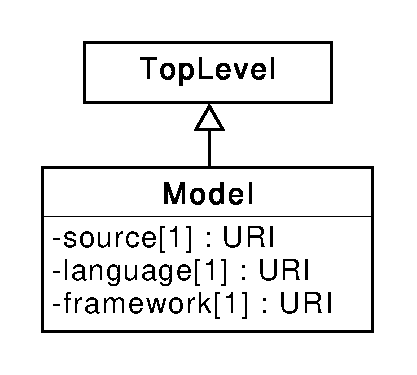
\includegraphics[scale=0.6]{uml/model}
\caption[]{Diagram of the \sbol{Model} class and its associated properties.}
\label{uml:model}
\end{center}
\end{figure}

SBOL's \sbol{Model} objects are placeholders that point to some external modeling mechanism, with some additional meta-data to enable better reasoning about the contents of that external mechanism.
In this way, there is minimal duplication of standardization efforts and users of SBOL can specify the quantitative function of \sbol{ModuleDefinition} objects in a well-developed language of their choice. 

Each \sbol{Model} object specifies the location of the actual content of a qualitative/quantitative model, the language the model is implemented with, the modeling framework and the model's role(s). 

\subsubsection*{ The \sbolheading{source} property}\label{sec:source}
This REQUIRED property is a URI that specifies the actual location of a qualitative or quantitative model.

\subsubsection*{ The \sbolheading{language} property}\label{sec:language}
This REQUIRED property is a URI that specifies the language the model is implemented with. 
Values for this URI are RECOMMENDED to be chosen from the EMBRACE Data and Methods (EDAM) ontology where possible. A few suggested model types and corresponding URI values are shown in \ref{tbl:model_types}.

\begin{table}[ht]
  \begin{edtable}{tabular}{ll}
    \toprule
    \textbf{Model Language} & \textbf{URI} \\
    \midrule
    SBML  & \url{http://identifiers.org/edam/format_2585}\\
    CellML		 & \url{http://identifiers.org/edam/format_3240}\\
    BioPAX    & \url{http://identifiers.org/edam/format_3156}\\
    \bottomrule
  \end{edtable}
  \caption{Some commonly used model languages and their corresponding URIs.}
  \label{tbl:model_types}
\end{table}


\subsubsection*{ The \sbolheading{framework} property}\label{sec:framework}
This REQUIRED property is a URI that specifies the modeling framework that a model is implemented within. 
Values for this URI are RECOMMENDED to be chosen from the SBO's modeling framework terms where possible. A few suggested model frameworks and corresponding URI values are shown in \ref{tbl:model_frameworks}.

\begin{table}[ht]
  \begin{edtable}{tabular}{ll}
    \toprule
    \textbf{Framework} & \textbf{URI} \\
    \midrule
    Continuous  & \url{http://identifiers.org/biomodels.sbo/SBO:0000062}\\
    Discrete & \url{http://identifiers.org/biomodels.sbo/SBO:0000063}\\
    \bottomrule
  \end{edtable}
  \caption{Example modelling frameworks and corresponding SBO terms.}
  \label{tbl:model_frameworks}
\end{table}

\subsubsection*{Serialization}

The serialization of \sbol{Model} objects has the following form:

\lstsetsbol
\begin{lstlisting}
<sbol:Model rdf:about="http://www.sbolstandard.org/examples/toogleswicth">
  ...
  [\emph{one}]         <sbol:source rdf:resource="..."/> [\emph{element}]
  [\emph{one}]         <sbol:language rdf:resource="..."/> [\emph{element}]
  [\emph{one}]         <sbol:framework rdf:resource="..."/> [\emph{element}]
</sbol:Model>
\end{lstlisting}

The example below shows the serialization of a \sbol{Model} object. The model object includes information about the models of a toggle switch. The model is implemented in SBML using a continuous modelling framework. The source property shows the physical location of the SBML model, in a model repository. 
\lstsetsbol
\begin{lstlisting}
<?xml version="1.0" ?>
<rdf:RDF xmlns:rdf="http://www.w3.org/1999/02/22-rdf-syntax-ns#" xmlns:sbol="http://sbols.org/v2#">
  <sbol:Model rdf:about="http://www.sbolstandard.org/examples/toogleswicth">
    <sbol:source rdf:resource="http://virtualparts.org/part/pIKE_Toggle_1"/>
    <sbol:language rdf:resource="http://identifiers.org/edam/format_2585"/>
    <sbol:framework rdf:resource="http://identifiers.org/biomodels.sbo/SBO:0000062"/>
  </sbol:Model>
</rdf:RDF>

\end{lstlisting}
\label{ser:Model}

\subsection{ModuleDefinition}
\label{sec:ModuleDefinition}

\Ctodo{This section has not been edited much compared to other sections. We need to explain classes and their properties a bit more in detail.}

\begin{figure}[ht]
\begin{center}
\includegraphics[scale=0.6]{uml/module_definition}
\caption[]{Diagram of the \sbol{ModuleDefinition} class and its associated properties.}
\label{uml:module_definition}
\end{center}
\end{figure}

The \sbol{ModuleDefinition} class is the hub where the structural and functional aspects of genetic designs come together to form a complete picture of the design. 
A \sbol{ModuleDefinition} object is composed from zero or more \sbol{FunctionalComponent}, \sbol{Module}, and \sbol{Interaction} objects, and links to zero or more \sbol{Model} objects. 
A \sbol{ModuleDefinition} object relies on the ``direction'' data fields of its \sbol{FunctionalComponent} objects to specify whether they serve as its inputs or outputs.
\Ctodo{the direction bit needs to be said much more clearly}

\subsubsection*{The \sbolheading{roles} property}\label{sec:roles}
This property is OPTIONAL and may include a set of URIs that specifies the intended use of a \sbol{ModuleDefinition} entity. 
These URIs may identify terms for abstract module roles, such as``inverter'' or ``AND gate'', or they may identify terms for purely biological roles, such as ``metabolic pathway'' and ``signaling cascade''.
\Ctodo{make this sentence clearer}

\Ctodo{Make these more paralell to componentdefinition in the way that they are written}
\subsubsection*{The \sbolheading{models} property}\label{sec:models}
This property is OPTIONAL and includes identities of associated \sbol{Model} entities.

SBOL's \sbol{Model} objects are used to link genetic descriptions of biological parts and their interactions to computational models.
A ModuleDefinition object can link to more than one model since each one can encode different levels of functional detail and play different roles in engineering design. 
\Ctodo{clarify this bit with a bit more explanation and better content}

\Ctodo{make sure submodules --> modules}

\subsubsection*{The \sbolheading{modules} property}\label{sec:modules}
This property is optional and includes a set of \sbol{Module} entities, which refer to \sbol{ModuleDefinition}s to be imported.
\Ctodo{use better language, like in componentdefinition}

\Ctodo{component --> functionalComponent in examples}
\subsubsection*{The \sbolheading{functionalComponents} property}
\label{sec:functionalComponents}
This property is optional and includes a set of \sbol{FunctionalComponent} entities. These entities are then used to describe biological interactions via \sbol{Participation} entities.

\Ctodo{use better language}

\subsubsection*{The \sbolheading{interactions} property}\label{sec:interactions}
This property is optional and includes a set of \sbol{Interaction} entities, which include \sbol{Participation} entities.

\subsubsection*{Serialization}

The serialization of \sbol{ModuleDefinition} has the following form:
\lstsetsbol
\begin{lstlisting}
<sbol:ModuleDefinition rdf:about="...">
               ...
  [\emph{zero or more}]  <sbol:role rdf:resource="..."/> [\emph{elements}]
  [\emph{zero or more}]  <sbol:model rdf:resource="..."/> [\emph{elements}]
  [\emph{zero or more}] <sbol:component>
                 <sbol:FunctionalComponent rdf:about="...">...</sbol:FunctionalComponent >
               </sbol:component> [\emph{elements}]
  [\emph{zero or more}] <sbol:subModule>
                 <sbol:Module rdf:about="...">...</sbol:Module>
               </sbol:subModule> [\emph{elements}]
  [\emph{zero or more}] <sbol:interaction>
                 <sbol:Interaction rdf:about="...">...</sbol:Interaction>
               </sbol:interaction> [\emph{elements}]
</sbol:ModuleDefinition>
\end{lstlisting}
\Ctodo{Is this template still correct, given ``subModule''?}

\Rtodo{Add an example, like for all the rest.  JSB: done, but needs to be sanity-checked since I created it by hand.}

The example below shows a simple \sbol{ModuleDefinition} containing two components, a \sbol{FunctionalComponent} for a DNA sequence encoding constitutive expression of GFP and another for the GFP protein expressed from this sequence, plus an interaction describing that relation.

\lstsetsbol
\begin{lstlisting}
  <sbol:ModuleDefinition rdf:about="http://sbolstandard.org/example/GFP_expression">
    <sbol:component>
      <sbol:FunctionalComponent rdf:about="http://sbolstandard.org/example/Constitutive_GFP">
        <sbol:definition rdf:resource="http://sbolstandard.org/example/GFP_generator"/>
        <sbol:access rdf:resource="http://sbols.org/v2#public"/>
        <sbol:direction rdf:resource="http://sbols.org/v2#none"/>
      </sbol:FunctionalComponent>
    </sbol:component>
    <sbol:component>
      <sbol:FunctionalComponent rdf:about="http://sbolstandard.org/example/GFP_protein">
        <sbol:definition rdf:resource="http://sbolstandard.org/example/GFP"/>
        <sbol:access rdf:resource="http://sbols.org/v2#public"/>
        <sbol:direction rdf:resource="http://sbols.org/v2#out"/>
      </sbol:FunctionalComponent>
    </sbol:component>
    <sbol:interaction>
      <sbol:Interaction rdf:about="http://sbolstandard.org/example/GPF_expression/interaction/express_GFP">
         ...
      </sbol:Interaction>
    </sbol:interaction>
  </sbol:ModuleDefinition>
\end{lstlisting}

\Rtodo{Should this be here or defined in ComponentInstance section?  JSB: here}

\subsubsection{FunctionalComponent}
\label{sec:FunctionalComponent}
Composition of the functional layer of SBOL designs is accomplished using \sbol{FunctionalComponent} objects. Each FunctionalComponent object is owned by a \sbol{ModuleDefinition} and serves as an explicit usage of a \sbol{Component} object for the purpose of fulfilling some function. 

\sbol{FunctionalComponent} derives from \sbol{ComponentInstance}, and therefore has the definition and access properties. Additionally, it has a \sbol{direction} property that specifies whether it serves as an input, output, both, or neither for the \sbol{ModuleDefinition} that contains it.

\Ctodo{Previously said a Module could own a FunctionalComponet, which i'm pretty sure is false -JB  Yes, it's false, fix it}

\paragraph{The \sbolheading{direction} property}\label{sec:direction}
Each \sbol{FunctionalComponent} MUST specify via the \sbol{direction} property whether it serves as an  input, output, both, or neither for its parent \sbol{ModuleDefinition} object. 
The value for this property MUST be one of the values given in \ref{tbl:functionalcomponent_directions}.


\LDtodo{Need to explain direction better.}


\begin{table}[ht]
  \begin{edtable}{tabular}{ll}
    \toprule
    \textbf{Direction URI} & \textbf{Description} \\
    \midrule
    \url{http://sbols.org/v2#inout}  & To indicate a \sbol{FunctionalComponent} can be used as both input or output\\
    \url{http://sbols.org/v2#in}  & To indicate a \sbol{FunctionalComponent} can be used as input\\
    \url{http://sbols.org/v2#out}  & To indicate a \sbol{FunctionalComponent} can be used as output\\
    \url{http://sbols.org/v2#none}  & To indicate a \sbol{FunctionalComponent} is neither input nor output\\
    \bottomrule
  \end{edtable}
  \caption{URIs for the \sbol{direction} property.}
  \label{tbl:functionalcomponent_directions}
\end{table}

\paragraph{Serialization}

The serialization of \sbol{FunctionalComponent}s has the following form.
\lstsetsbol
\begin{lstlisting}
<sbol:FunctionalComponent rdf:about="...">
  [\emph{zero or one}]   <sbol:definition rdf:resource="..."/> [\emph{element}]
  [\emph{one}]           <sbol:access rdf:resource="..."/> [\emph{element}]
  [\emph{one}]           <sbol:direction rdf:resource="..."/> [\emph{element}]
  [\emph{zero or more}]  <sbol:mapsTo rdf:resource="..."/> [\emph{elements}]
</sbol:FunctionalComponent>
\end{lstlisting}

In the example below, the functional component is defined as public input or output. The component refers to the \texttt{Part:BBa\_R0010} promoter from the Parts Registry.
\lstsetsbol
\begin{lstlisting}
<sbol:FunctionalComponent rdf:about="http://sbolstandard.org/example/laci_inverter/fc/Part:BBa_R0010">
  <sbol:definition rdf:resource="http://www.partsregistry.org/Part:BBa_R0010"/>
  <sbol:access rdf:resource="http://sbols.org/v2#public"/>
  <sbol:direction rdf:resource="http://sbols.org/v2#inout"/>
</sbol:FunctionalComponent>
\end{lstlisting}

\subsubsection{Module}
\label{sec:Module}

\begin{figure}[ht]
\begin{center}
\includegraphics[scale=0.6]{uml/module}
\caption[]{Diagram of the \sbol{Module} class and its associated properties.}
\label{uml:module}
\end{center}
\end{figure}

The \sbol{Module} class enables the composition of \sbol{ModuleDefinition} objects from other, smaller \sbol{ModuleDefinition} objects. \textcolor{red}{The first data field, ``definition'', links to the ModuleDefinition object that is effectively a part of the Module object that owns the Module object.} The second data field, ``mappings'', is a set of MapsTo objects that link between the Component objects at the same level of the design hierarchy as the Module object and the Component objects that are lower in the design hierarchy, thereby composing these objects with greater specificity.

\Ctodo{mappings or mapsTo? --> mapsTo} 
\Ctodo{need to clean up this whole description}
\Ctodo{Is the notion of ``level of design hierarchy'' real?  I think it doesn't need to be stated here, it's actually a best practice. -->  it's a best practice.  Nick will write this better.}

\paragraph{Serialization}
The serialization of \sbol{Module}s has the following form.
\lstsetsbol
\begin{lstlisting}
<sbol:Module rdf:about="...">
  [\emph{one}]          <sbol:definition rdf:resource="..."/>[\emph{element}]
  [\emph{zero or more}] <sbol:mapping>
                 <sbol:MapsTo rdf:about="...">...</sbol:MapsTo>
               </sbol:mapping> [\emph{element}]
</sbol:Module>
\end{lstlisting}

The example below specifies a TetR inverter that is being used as
a part of a toggle switch:

\lstsetsbol
\begin{lstlisting}
<sbol:Module rdf:about="http://sbolstandard.org/example/toggle_switch/submodule/tetr_inverter">
  <sbol:definition rdf:resource="http://sbolstandard.org/example/tetr_inverter"/>
</sbol:Module>
\end{lstlisting}

\Rtodo{add an example; JSB: done}

\subsubsection{MapsTo}
\label{sec:MapsTo}

\begin{figure}[ht]
\begin{center}
\includegraphics[scale=0.6]{uml/maps_to}
\caption[]{Diagram of the \sbol{MapsTo} class and its associated properties.}
\label{uml:maps_to}
\end{center}
\end{figure}
The \sbol{MapsTo} class serves as a means of linking between \sbol{ComponentInstance} objects (both \sbol{Component}s and \sbol{FunctionalComponent}s) at different levels of the design hierarchy. For example, when a child \sbol{ModuleDefinition} object is instantiated inside a parent \sbol{ModuleDefinition} object, a \sbol{MapsTo} object is used to link these two ModuleDefinitions. MapsTo has properties to specify components from the parent and child entities, and also to specify how these components are linked.

\Ctodo{need to explain the whole 3-way mapsto model and importation better}

\paragraph{The \sbolheading{local} property}\label{sec:local}
This required property is used to specify the \sbol{ComponentInstance} from the parent entity.

\paragraph{The \sbolheading{remote} property}\label{sec:remote}
This required property is used to specify the \sbol{ComponentInstance} from the child entity being imported by the parent.

\paragraph{The \sbolheading{refinement} property}\label{sec:refinement}
Each \sbol{MapsTo} entity must also specify the relationship between its local and remote components using the refinement property. The Table \ref{tbl:mapsto_refinement} lists the values 

\begin{table}[ht]
  \begin{edtable}{tabular}{lp{4in}}
    \toprule
    \textbf{Refinement URI} & \textbf{Description} \\
    \midrule
    \url{http://sbols.org/v2#useremote}  & Indicates that \sbol{ComponentInstance} from the child entity is used in the parent, instead of the \sbol{ComponentInstance} specified in the parent entity.\\
    \url{http://sbols.org/v2#uselocal}  & Indicates that \sbol{ComponentInstance} from the parent entity is used in the parent instead of the imported the \sbol{ComponentInstance} child entity.\\
    \url{http://sbols.org/v2#verifyIdentical}  & Indicates that ComponentInstance entities must link to the same \sbol{ComponentDefinition} object\\
        \url{http://sbols.org/v2#merge}  & Indicates that data fields of the local and remote ComponentInstantiation entities are to be interpreted in combination\\
    \bottomrule
  \end{edtable}
  \caption{URIs for the \sbol{refinement} property.}
  \label{tbl:mapsto_refinement}
\end{table}

\Ctodo{libsbol and refinements types here need to agree on consistent capitalization. GM: We agreed to start with lowercase and use the Capital for the next word.}
\Ctodo{The notion of refinement is very unclear -JB  Clean up the text}

%GM: The paragraph below is now explained in the table above. Commented for now. Please remove the commented lines if you agree with the table description.
%In addition to specifying a link, each MapsTo object must also specify a ``refinement'' relationship between its local and remote Components. Under this data model, there are four types of refinement: ``verifyIdentical'' requires that the Component objects link to the same ComponentDefinition object, ``useLocal'' indicates that the local Component object overrides the remote Component object, ``useRemote'' indicates the opposite, and “merge” indicates that data fields of the local and remote ComponentInstantiation objects are to be interpreted in combination.


%\begin{figure}[ht]
%\begin{center}
%\includegraphics[scale=0.6]{images/MapsTo_Diagram1}
%\caption{Linking Components using MapsTo entities.}
%\label{image:maps_to_diagram1}
%\end{center}
%\end{figure}

\begin{figure}[ht]
\begin{center}
\includegraphics[scale=1]{images/MapsTo_Diagram2}
\caption{Linking Components using \sbol{MapsTo} entities. Boxed with the C label represent Component entities and boxes with the M label represent \sbol{MapsTo} entities.}
\label{image:maps_to_diagram2}
\end{center}
\end{figure}
\Ctodo{Caption: why are some RBSs not filled in?}

An example design of a \sbol{ComponentDefinition} using \sbol{MapsTo} entities is shown at the left hand side of the Figure \ref{image:maps_to_diagram2}. The resulting entity is formed of a promoter, a RBS and a CDS. 
Three sub components to create the design includes: a promoter-RBS \sbol{ComponentDefinition} with a RBS placeholder without detailed definition; a RBS \sbol{ComponentDefinition} with full description; and a RBS-CDS \sbol{ComponentDefinition} with a RBS placeholder, which is also not defined in full detail. 
In the figure, boxes with the C label represent \sbol{Component} entities and boxes with the M label represent the \sbol{MapsTo} entities.
In the design RBSs that are not fully defined are replaced with another RBS \sbol{ComponentDefinition} (displayed in green colour). \sbol{MapsTo} entities attached to sub components for promoter-RBS and RBS-CDS \sbol{ComponentDefinition}s include the ``use local'' refinement to replace RBSs with the fully defined version. In the second design at the right hand side of the figure, \sbol{MapsTo} entities are used to import the RBS from the promoter-RBS \sbol{ComponentDefinition} overwriting the RBS in RBS-CDS \sbol{ComponentDefinition}. 

\Ctodo{Need to expand this explanation a bit more to drive home the points -JB}

\paragraph{Serialization}
The serialization of \sbol{MapsTo} has the following form.
\lstsetsbol
\begin{lstlisting}
<sbol:MapsTo rdf:about="...">
  [\emph{one}] <sbol:refinement>...</sbol:refinement> [\emph{element}]
  [\emph{one}] <sbol:remote rdf:resource="..."/> [\emph{element}]]
  [\emph{one}] <sbol:local rdf:resource="..."/> [\emph{element}]]
</sbol:MapsTo>
\end{lstlisting}

In the example below, a \sbol{FunctionalComponent} entity from the submodule is linked to a \sbol{FunctionalComponent} entity in a parent module. The former is described in the imported \sbol{ModuleDefinition} entity which is referred to by the definition property of the \sbol{Module} entity. The latter is defined in the parent \sbol{ModuleDefinition}, importing the sub module. The full example can be found in \ref{ser:toggleswitch}.
\lstsetsbol
\begin{lstlisting}
<sbol:MapsTo rdf:about="http://sbolstandard.org/example/toggle_switch/submodule/laci_inverter/mapping/Q6QR72">
  <sbol:refinement>USEREMOTE</sbol:refinement>
  <sbol:remote rdf:resource="http://sbolstandard.org/example/toggle_switch/fc/Q6QR72"/>
  <sbol:local rdf:resource="http://sbolstandard.org/example/tetr_inverter/fc/Q6QR72"/>
</sbol:MapsTo>
\end{lstlisting}



\subsubsection{Interaction}
\label{sec:Interaction}

\begin{figure}[ht]
\begin{center}
\includegraphics[scale=0.6]{uml/interaction}
\caption[]{Diagram of the \sbol{Interaction} class and its associated properties.}
\label{uml:interaction}
\end{center}
\end{figure}

\Ctodo{Some of this description is incorrect or unclear}
The Interaction class provides a qualitative basis for asserting the intended function of a given ModuleDefinition object. The proposed data model supports the representation of regulatory interactions, such as activation or repression, and processes from the central dogma of biology, such as transcription and translation. Other supported interaction types include non-covalent binding between a small molecule and TF, and phosphorylation of a TF by an enzyme. 
\Ctodo{What does it mean for an interaction to be supported? --> nothing, pick a better word}

Each Interaction object must specify its type with at least one URI that identifies an appropriate ontology term, such as a term from the Systems Biology Ontology (SBO). If an Interaction object has multiple type URIs, then they must identify synonymous terms. 

\Ctodo{Like the others, SBO is REQUIRED if the term exists, and you can add other stuff.  We also need to explain this up front in the beginning of the section}

Furthermore, an\sbol{Interaction} object can specify the set of \sbol{FunctionalComponent} entities that are interacting by linking to \sbol{Participation} objects that descibe how each one participates in the interaction.
\Rtodo{I don't think this is really a MUST.  JSB: it wasn't; it is resolved.}

\paragraph{Serialization}

The serialization of \sbol{Interaction}s has the following form.
\lstsetsbol
\begin{lstlisting}
<sbol:Interaction rdf:about="...">
  [\emph{one or more}] <sbol:type rdf:resource="..."/> [\emph{elements}]
  [\emph{one or more}] <sbol:participation>
                <sbol:Participation rdf:about="...">...</sbol:Participation>
              </sbol:participation> [\emph{elements}]
</sbol:Interaction>
\end{lstlisting}

\begin{figure}[ht]
\begin{center}
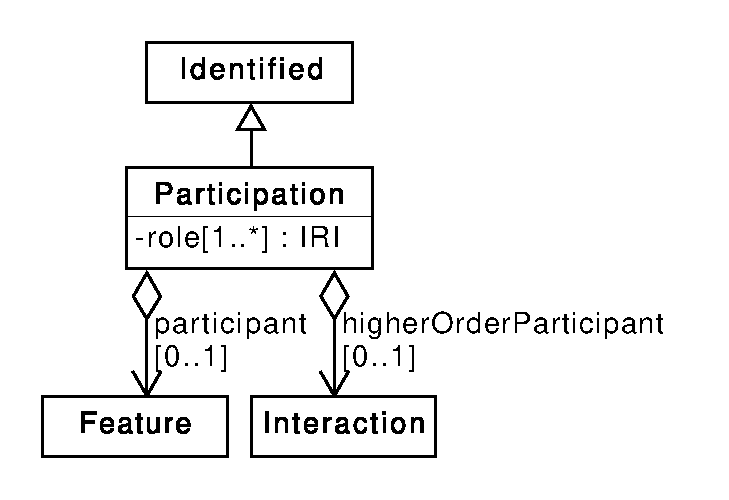
\includegraphics[scale=0.6]{uml/participation}
\caption[]{Diagram of the \sbol{Participation} class and its associated properties.}
\label{uml:participation}
\end{center}
\end{figure}

\subsubsection{Participation}
\label{sec:Participation}

\Ctodo{Fix the linking and clean grammar}

Each object of the Participation class must specify the role of its participant FunctionalComponent object in its parent Interaction object with at least one URI that identifies an appropriate ontology term. If a Participation object has multiple role URIs, then they must identify synonymous terms. 

\Ctodo{SBO is our REQUIRED term if available, just as in the prior cases}

\Ctodo{Goksel is going to check if there is a superset ontology that should displace SBO}

While the Interaction class provide a qualitative description of genetic function, quantitative descriptions are also needed for genetic design. Instead of introducing a new language for the specification of mathematical models of biology, the proposed data model leverages existing standards and links to them via the Model class. 

\paragraph{Serialization}

The serialization of \sbol{Participation}s has the following form.
\lstsetsbol
\begin{lstlisting}
<sbol:Participation rdf:about="...">
  [\emph{one or more}] <sbol:role rdf:resource="..."/>
  [\emph{one or more}] <sbol:participant rdf:resource="..."/>
</sbol:Participation>
\end{lstlisting}

In the example below, the role of participating \sbol{FunctionalComponent} is defined to be \external{inhibitor}, using the \external{SBO:0000020} term. This component is specified using the participant property of the \sbol{Participation} entity.
\lstsetsbol
\begin{lstlisting}
<sbol:Participation rdf:about="http://sbolstandard.org/example/laci_inverter/interaction/LacI_pLacI/participation/P03023">
  <sbol:role rdf:resource="http://identifiers.org/biomodels.sbo/SBO:0000020"/>
  <sbol:participant rdf:resource="http://sbolstandard.org/example/laci_inverter/fc/P03023"/>
</sbol:Participation>
\end{lstlisting}

\subsection {Collection}
\label{sec:Collection}
The \sbol{Collection} class is a class that groups together a set of \sbol{TopLevel} objects that have something in common. 
Some examples of \sbol{Collection} objects:
\begin{itemize}
\item Results of a query to find all \sbol{ComponentDefinition} objects that function as promoters in a repository.
\item A set of \sbol{ModuleDefinition} objects representing a library of NAND gates.
\item A \sbol{ModuleDefinition} for a complex design, and all of the \sbol{ModuleDefinition}, \sbol{ComponentDefinition}, \sbol{Sequence}, and \sbol{Model} objects used to provide its full specification.
\end{itemize}

\begin{figure}[ht]
\begin{center}
\includegraphics[scale=0.6]{uml/collection}
\caption[]{Diagram of the \sbol{Collection} class and its associated properties.}
\label{uml:collection}
\end{center}
\end{figure}

\subsubsection*{The \sbolheading{members} property}
The \sbol{members} property has a data type of URI and has the URI for a \sbol{TopLevel} entity.  A collection may have any number of members, including none.

\subsubsection*{Serialization}

The serialization of \sbol{Collection} objects has the following form:

\lstsetsbol
\begin{lstlisting}
<sbol:Collection rdf:about="...">
              ...
  [\emph{one or more}] <sbol:member rdf:resource="..."/> [\emph{element}]
</sbol:Collection>
\end{lstlisting}

\Ctodo{We should make all of the example URIs compliant}

The example below shows the serialization of a \sbol{Collection} object grouping together a library of constitutive promoters.
\lstsetsbol
\begin{lstlisting}
<?xml version="1.0" ?>
<rdf:RDF xmlns:rdf="http://www.w3.org/1999/02/22-rdf-syntax-ns#" xmlns:dcterms="http://purl.org/dc/terms/" xmlns:sbol="http://sbols.org/v2#">
  <sbol:Collection rdf:about="http://parts.igem.org/Promoters/Catalog/Anderson">
    <sbol:displayId>Anderson</sbol:displayId>
    <dcterms:title>Anderson promoters</dcterms:title>
    <dcterms:description> The Anderson promoter collection</dcterms:description>
    <sbol:member rdf:resource="http://parts.igem.org/wiki/index.php/Part:BBa_J23119"/>
    ...
    <sbol:member rdf:resource="http://parts.igem.org/wiki/index.php/Part:BBa_J23118"/>
  </sbol:Collection>
</rdf:RDF>

\end{lstlisting}
\label{ser:Collection}

\subsection{Extending the SBOL Representation:  Annotations}
\label{sec:Annotations}
\label{sec:annotations}

\Rtodo{Matthew/Goksel/Jake: please review.}

SBOL does not attempt to represent all information about a biological system, since many things do not yet have a clear ``right way'' to be represented, such as design intent, biological context, or performance data.  Instead, SBOL allows the embedding of application specific data that are not captured by the SBOL standard.  Such data are optional, but can be computationally generated and exchanged via SBOL documents without getting lost. 

To do this, SBOL provides an ``annotation'' mechanism for attaching arbitrary information to SBOL objects, which allows SBOL models to be connected with any other models in an extensible manner.
In particular, three methods are supported for connecting the SBOL data model with other, possibly application-specific data:
\begin{enumerate}
\item Information that is ``part'' of an SBOL object (i.e., a ``filled diamond'' relationship) is annotated simply by adding non-conflicting properties and custom entries to an SBOL object.  An example might be source information about the registry from which a \sbol{ComponentDefinition} was imported.
\item Information that is an independent object is annotated by wrapping it inside of a \sbol{GenericTopLevel} object.  An example might be a data sheet describing the performance of a \sbol{ModuleDefinition} in some particular context.
\item Conversely, rather than embedding external objects in SBOL, SBOL objects can also be linked to external data.  The only requirement is that some URI resolution mechanism must be available that allows the links from SBOL objects to be followed when needed.
\end{enumerate}

\subsubsection{Annotating SBOL objects}
% whole set of labels for the properties defined herein
\label{sec:value}
\label{sec:Annotation}
\label{sec:AnnotationValue}
\label{sec:ListOfAnnotations}

Each \sbol{Identified} object may have a number of annotations in the form of name/value property pairs. The \sbol{name} property is specified by a qualified name (\external{QName}), which is composed of a namespace, a prefix, and a local name. The \sbol{value} property can be of type \external{String}, \external{URI}, or \external{ListOfAnnotations}. The \external{ListOfAnnotations} is composed of a \sbol{nestedQName}, \sbol{nestedURI}, and a list of nested \sbol{annotations}.

\Ctodo{NIC: Please update UML as follows: remove link from Identifed to AnnotationValue, change type of name to QName, change label of Literal box to String, add new class ListOfAnnotations that inherits from AnnotationValue with properties nestedQName : QName, nestedURI : URI, and a 0..* annotations link to the Annotation class.}

\begin{figure}[!ht]
\begin{center}
\includegraphics[scale=0.6]{uml/identified_annotations}
\caption[]{Diagram of the \sbol{Annotation} class and its association with \sbol{Identified} and \sbol{AnnotationValue} objects, which is used for annotating SBOL entities with application specific data.}
\label{uml:identified_annotations}
\end{center}
\end{figure}

\paragraph{Serialization}
The ComponentDefinition example for a promoter serialized below shows how annotations can be added to SBOL objects. Annotations are added using the relevant information from the Parts Registry. Annotation property names are qualified with the \external{http://www.partsregistry.org/} namespace, which is prefixed using \external{pr}. The first annotation is named as \external{pr:group}, indicating the iGEM group designing the promoter, and has a \external{String} value. The second \external{pr:experience} annotation has a \external{URI} value and is serialised as an RDF resource pointing to the information Web page on the Parts Registry for the promoter. The  \external{pr:information} property represents a complex annotation which is a type of \external{pr:Information} and includes information about the regulatory details of the promoter using Parts Registry categories.   

\begin{figure} [ht]
\lstsetsbol
\begin{lstlisting}
<?xml version="1.0" ?>
<rdf:RDF xmlns:pr="http://www.partsregistry.org/" xmlns:rdf="http://www.w3.org/1999/02/22-rdf-syntax-ns#" xmlns:dcterms="http://purl.org/dc/terms/" xmlns:sbol="http://sbols.org/v2#">
  <sbol:ComponentDefinition rdf:about="http://www.partsregistry.org/Part:BBa_J23119">
    <pr:group>iGEM2006_Berkeley</pr:group>
    <pr:experience rdf:resource="http://www.partsregistry.org/Part:BBa_J23119:Experience"/>
    <pr:information>
      <pr:Information rdf:about="http://parts.igem.org/cgi/partsdb/part_info.cgi?part_name=BBa_J23119">
        <pr:sigmafactor>//rnap/prokaryote/ecoli/sigma70</pr:sigmafactor>
        <pr:regulation>//regulation/constitutive</pr:regulation>
      </pr:Information>
    </pr:information>
    <dcterms:title>J23119</dcterms:title>
    <dcterms:description>Constitutive promoter</dcterms:description>
    <sbol:type rdf:resource="http://www.biopax.org/release/biopax-level3.owl#DnaRegion"/>
    <sbol:role rdf:resource="http://purl.org/obo/owl/SO#SO_0000167"/>
  </sbol:ComponentDefinition>
</rdf:RDF>
\end{lstlisting}
\label{ser:Annotation}
\end{figure}




\subsubsection{GenericTopLevel}  
\label{sec:GenericTopLevel}
SBOL documents can also be annotated at the top level. 
SBOL's \sbol{GenericTopLevel} is a top-level entity whose only purpose is to include a set of annotations as described above. 
Entities that have independent existence (i.e., would be another ``top level'' class) and are not recognised by the SBOL standard are loaded into these top level entities. 
These \sbol{GenericTopLevel} entities can thus be safely used by tools to exchange non-SBOL data embedded separately within SBOL.
As with any other top level entities, \sbol{GenericTopLevel} entities may include SBOL properties such as \sbol{name}, \sbol{description}, \sbol{displayId} and so on. The type of data found in the generic entity is indicated using the standard \external{rdf:type} property.

\begin{figure}[ht]
\begin{center}
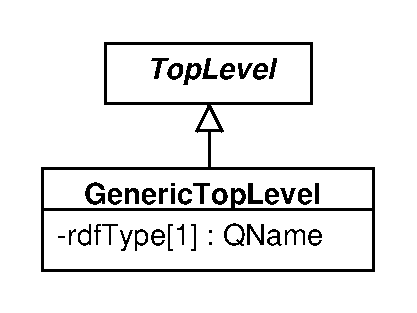
\includegraphics[scale=0.6]{uml/generictoplevel}
\caption[]{Diagram of the \sbol{GenericTopLevel} class and its associated properties, which is used for embedding externally defined entities into SBOL documents.}
\label{uml:generictoplevel}
\end{center}
\end{figure}

The example below shows how a datasheet object can be added to an SBOL document using the \sbol{GenericTopLevel} class. 
The J23119 promoter example is annotated with the URI of a top Level Datasheet object, here defining the annotation properties using the custom \external{\path{http://www.myapp.org/}} namespace and the \external{myapp} prefix. 
The datasheet object, with the data type of \external{myapp:Datasheet}, is accessed using the \external{URI} value specified by the \external{myapp:characterizationData} property of the promoter component definition. 
The datasheet object is further annotated with the transcription rate and the URI for the actual characterization data using the \external{myapp:transcriptionRate} and \external{myapp:characterizationData} properties respectively.
Finally, this data sheet is linked from the component is describes using an annotation with a \external{myapp:datasheet} property whose value is the data sheet's URI.

\begin{figure}[ht]
\lstsetsbol
\begin{lstlisting}
<?xml version="1.0" ?>
<rdf:RDF xmlns:myapp="http://www.myapp.org/" xmlns:rdf="http://www.w3.org/1999/02/22-rdf-syntax-ns#" xmlns:dcterms="http://purl.org/dc/terms/" xmlns:sbol="http://sbols.org/v2#">
  <sbol:ComponentDefinition rdf:about="http://www.partsregistry.org/Part:BBa_J23119">
    <myapp:datasheet rdf:resource="http://www.myapp.org/datasheet/1"/>
    <dcterms:title>J23119</dcterms:title>
    <dcterms:description>Constitutive promoter</dcterms:description>
    <sbol:type rdf:resource="http://www.biopax.org/release/biopax-level3.owl#DnaRegion"/>
    <sbol:role rdf:resource="http://purl.org/obo/owl/SO#SO_0000167"/>
  </sbol:ComponentDefinition>
  <myapp:Datasheet rdf:about="http://www.myapp.org/datasheet/1">
    <myapp:characterizationData rdf:resource="http://www.myapp.org/measurement/1"/>
    <myapp:transcriptionRate>1</myapp:transcriptionRate>
    <dcterms:title>Datasheet 1</dcterms:title>
  </myapp:Datasheet>
</rdf:RDF>

\end{lstlisting}
\label{ser:GenericTopLevel}
\end{figure}